\section{Auswertung}

Die Temperatur wurde nicht direkt gemessen, sondern es wurde ein Widerstandstermometer verwendet.
Die gemessenen Widerstände können mithilfe der \autoref{fig:abb3} in eine Temperatur umgerechnet werden.
\begin{figure}[H]
  \centering
  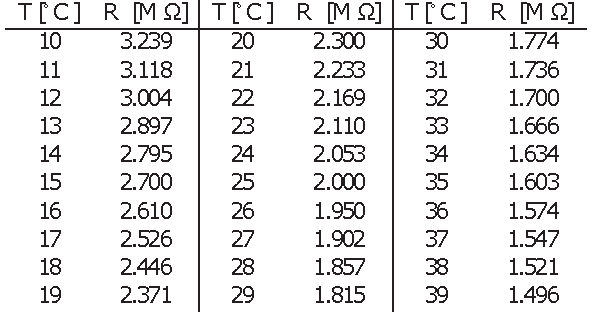
\includegraphics{figures/Temperatur.pdf}
  \caption{Temperatur der Luft bei verschiedenen Widerständen \cite{ap12}\, .} 
  \label{fig:abb3}
\end{figure}
Die Viskusität von Luft kann durch die \autoref{fig:viskositaet} bestimmt werden.
\begin{figure}[H]
  \centering
  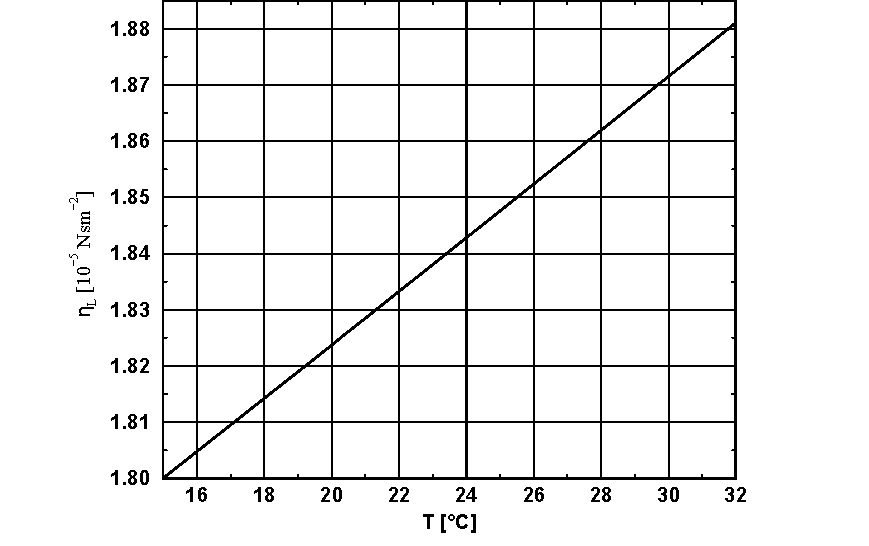
\includegraphics{figures/Viskositaet.pdf}
  \caption{Die Viskosität von Luft bei verschiedenen Temperaturen  \cite{ap12}\, .} 
  \label{fig:viskositaet}
\end{figure}


Um die Ladung der Öltröpfchen zu ermitteln, wurden Messungen bei fünf verschiedenen Spannungen für jeweils fünf Tröpfchen durchgeführt.
Alle Zeiten wurden für eine Strecke von $s = 5 \, \unit{\milli\meter}$ gemessen.
Die Widerstände können aufgrund der Genauigkeit des Geräts nur auf zwei Nachkommastellen abgelesen werden, zur Temperaturermittlung
müssen also entsprechende Rundungen getroffen werden. \\

Dabei übersetzen sich die gemessenen Widerstände wie folgt in Temperaturen und Viskositäten:
\begin{align*}
  R &= 1,99 \,\si{\mega\ohm} \Leftrightarrow T = 25 \,\si{\celsius} \Leftrightarrow \eta_\text{L} = 1,8475 \cdot 10^{-5} \,\unit{\newton} \unit{\dfrac{\second}{\meter^2}} \Leftrightarrow R = 1,98 \, \si{\mega\ohm} \\
  R &= 1,97 \,\si{\mega\ohm} \Leftrightarrow T = 26 \,\si{\celsius} \Leftrightarrow \eta_\text{L} = 1,8525 \cdot 10^{-5} \,\unit{\newton} \unit{\dfrac{\second}{\meter^2}} \,.
\end{align*}
\begin{table}[H]
    \caption{Messdaten der Öltröpfchen für verschiedene Spannungen $U$.}
    \label{tab:t_werte}
        \begin{tabular}{c c c c c}
            \begin{tabular}{S S[table-format=1.3] S[table-format=1.3]}
              %\caption{Messdaten bei $R = 1,99 \,\si{\mega\ohm}$, $U = 157 \,\si{\volt}$.}
              \toprule
              {Teilchen} & {$ t_{ab} \mathbin{/} \unit{\second}$} & {$ t_{auf} \mathbin{/} \unit{\second}$}\\
              \midrule
              1      &     6.690     &     3.612       \\
                     &     3.422     &     6.297       \\
                     &     7.938     &     5.690       \\
              2      &     4.04      &     4.44        \\
                     &     4.97      &     4.20        \\
                     &     4.53      &     4.71        \\
              3      &     4.44      &     5.98        \\
                     &     4.32      &     5.43        \\
                     &     4.15      &     5.34        \\
              4      &     4.85      &     5.64        \\
                     &     9.31      &     8.49        \\
                     &     7.02      &     8.75        \\
              5      &     3.86      &     4.37        \\
                     &     3.85      &     4.11        \\
                     &     3.75      &     4.35        \\
              \bottomrule
            \end{tabular}
            \begin{tabular}{S S[table-format=1.3] S[table-format=1.2]}
              %\caption{Messdaten bei $R = 1,99 \,\si{\mega\ohm}$, $U = 175 \,\si{\volt}$.}
              \toprule
              {Teilchen}&{$ t_{ab} \mathbin{/} \unit{\second}$} & {$ t_{auf} \mathbin{/} \unit{\second}$}\\
              \midrule
              6       &     3.73      &      3.02     \\
                      &     4.20      &      3.23     \\
                      &     4.63      &      3.47     \\
              7       &     3.43      &      4.13     \\
                      &     3.08      &      4.42     \\
                      &     3.52      &      4.11     \\
              8       &     3.12      &      3.03     \\
                      &     3.30      &      3.85     \\
                      &     2.49      &      2.77     \\
              9       &     3.06      &      2.85     \\
                      &     2.86      &      3.23     \\
                      &     3.20      &      2.97     \\
              10      &     2.09      &      2.14     \\
                      &     2.21      &      2.51     \\
                      &     2.43      &      1.98     \\
              \bottomrule
            \end{tabular}
            \begin{tabular}{S S[table-format=1.3] S[table-format=1.2]}
              %\caption{Messdaten bei $R = 1,98 \,\si{\mega\ohm}$, $U = 200 \,\si{\volt}$.}
              \toprule
              {Teilchen}&{$ t_{ab} \mathbin{/} \unit{\second}$} & {$ t_{auf} \mathbin{/} \unit{\second}$}\\
              \midrule
              11      &      3.32     &      3.43      \\
                      &      3.86     &      3.92      \\
                      &      3.61     &      3.24      \\
              12      &      3.52     &      3.82      \\
                      &      3.90     &      3.85      \\
                      &      3.63     &      3.85      \\
              13      &      2.75     &      2.67      \\
                      &      2.02     &      2.36      \\
                      &      2.44     &      2.54      \\
              14      &      4.54     &      5.10      \\
                      &      4.40     &      4.90      \\
                      &      4.47     &      4.77      \\
              15      &      2.30     &      1.67      \\
                      &      1.90     &      2.10      \\
                      &      2.05     &      2.11      \\
              \bottomrule
            \end{tabular} \\

            \begin{tabular}{S S[table-format=1.3] S[table-format=1.2]}
              %\caption{Messdaten bei $R = 1,98 \,\si{\mega\ohm}$, $U = 225 \,\si{\volt}$.}
              %\toprule
              {Teilchen}&{$ t_{ab} \mathbin{/} \unit{\second}$} & {$ t_{auf} \mathbin{/} \unit{\second}$}\\
              \midrule
                16      &     1.89      &      1.96     \\
                        &     1.88      &      1.95     \\
                        &     2.05      &      1.75     \\
                17      &     1.33      &      1.37     \\
                        &     1.97      &      2.05     \\
                        &     1.49      &      1.38     \\
                18      &     2.94      &      3.39     \\
                        &     3.13      &      3.37     \\
                        &     3.14      &      3.29     \\
                19      &     3.19      &      3.10     \\
                        &     2.99      &      3.56     \\
                        &     3.15      &      3.07     \\
                20      &     2.93      &      2.88     \\
                        &     2.70      &      2.95     \\
                        &     2.73      &      3.00     \\
              \bottomrule
            \end{tabular} 
            \begin{tabular}{S S[table-format=1.3] S[table-format=1.2]}
              %\caption{Messdaten bei $R = 1,97 \,\si{\mega\ohm}$, $U = 250 \,\si{\volt}$.}
              %\toprule
              {Teilchen}&{$ t_{ab} \mathbin{/} \unit{\second}$} & {$ t_{auf} \mathbin{/} \unit{\second}$}\\
              \midrule
                21      &     2.04      &      2.27     \\
                        &     2.15      &      2.12     \\
                        &     2.08      &      2.06     \\
                22      &     2.29      &      2.33     \\
                        &     2.08      &      2.25     \\
                        &     1.98      &      2.36     \\
                23      &     4.12      &      4.29     \\
                        &     3.23      &      3.90     \\
                        &     4.02      &      4.33     \\
                24      &     3.13      &      3.26     \\
                        &     2.80      &      3.51     \\
                        &     3.09      &      3.29     \\
                25      &     2.27      &      2.63     \\
                        &     2.67      &      2.93     \\
                        &     3.03      &      3.04     \\
              \bottomrule
            \end{tabular}
          \end{tabular}
\end{table}
Mit dem Zeit-Weg-Gesetzt \eqref{eq:Zeitweg}
\begin{equation*}
  v = \dfrac{s}{t}
  \label{eq:Zeitweg}
\end{equation*}

wird die Geschwindigkeit der von jedem einzelnen Tröpfchen bestimmt.
Die Geschwindigkeit sind in \autoref{tab:geschw} aufgetragen.
\begin{table}[H]
  \caption{Geschwindigkeiten der Öltröpfchen für verschiedene Spannungen}
  \label{tab:geschw}
  \centering
  \begin{subtable}[t]{0.45\textwidth}
      \small
      \subcaption{Daten für $U=\qty{157}{\volt}$}
      \label{stab:v157}
      \begin{table}[H]
          \centering
          \begin{tabular}{S S S}
            \toprule
              {Nr}& {$ v_{ab} \mathbin{/} \dfrac{\unit{\micro\meter}}{\unit{\second}}$}&{$ v_{auf} \mathbin{/} \dfrac{\unit{\micro\meter}}{\unit{\second}}$}\\
            \midrule
            
            \bottomrule
          \end{tabular}
        \end{table}
      
  \end{subtable}\qquad
  \begin{subtable}[t]{0.45\textwidth}
      \small
      \subcaption{Daten für $U=\qty{175}{\volt}$}
      \label{stab:v175}
      \begin{table}[H]
          \centering
          \begin{tabular}{S S S}
            \toprule
            {Nr}& {$ v_{ab} \mathbin{/} \dfrac{\unit{\micro\meter}}{\unit{\second}}$}&{$ v_{auf} \mathbin{/} \dfrac{\unit{\micro\meter}}{\unit{\second}}$}\\
            \midrule
            
            \bottomrule
          \end{tabular}
        \end{table}
      
  \end{subtable}\qquad
  \begin{subtable}[t]{0.45\textwidth}
      \small
      \subcaption{Daten für $U=\qty{200}{\volt}$}
      \label{stab:v200}
      \begin{table}[H]
          \centering
          \begin{tabular}{S S S}
            \toprule
            {Nr}& {$ v_{ab} \mathbin{/} \dfrac{\unit{\micro\meter}}{\unit{\second}}$}&{$ v_{auf} \mathbin{/} \dfrac{\unit{\micro\meter}}{\unit{\second}}$}\\
            \midrule
            
            \bottomrule
          \end{tabular}
        \end{table}
      
  \end{subtable}\qquad
  \begin{subtable}[t]{0.45\textwidth}
      \small
      \subcaption{Daten für $U=\qty{225}{\volt}$}
      \label{stab:v225}
      \begin{table}[H]
          \centering
          \begin{tabular}{S S S}
            \toprule
              {Nr}& {$ v_{ab} \mathbin{/} \dfrac{\unit{\micro\meter}}{\unit{\second}}$}&{$ v_{auf} \mathbin{/} \dfrac{\unit{\micro\meter}}{\unit{\second}}$}\\
            \midrule
            
            \bottomrule
          \end{tabular}
        \end{table}
      
  \end{subtable}\qquad
  \begin{subtable}[t]{0.45\textwidth}
      \small
      \subcaption{Daten für $U=\qty{250}{\volt}$}
      \label{stab:v250}
      \begin{table}[H]
          \centering
          \begin{tabular}{S S S}
            \toprule
              {Nr}& {$ v_{ab} \mathbin{/} \dfrac{\unit{\micro\meter}}{\unit{\second}}$}&{$ v_{auf} \mathbin{/} \dfrac{\unit{\micro\meter}}{\unit{\second}}$}\\
            \midrule
            
            \bottomrule
          \end{tabular}
        \end{table}
  \end{subtable}
\end{table}

Die Ladungen der Tröpfchen sind in \autoref{tab:Ladungen} aufgetragen. Dazu muss zunächst die effektive Viskosität mit \eqref{eq:Veff}, der Radius der Tröpfchen \eqref{eq:rmitEfled} und die korrigierte Ladung \eqref{eq:qKorr} berechnet werden.

\begin{table}[H]
  \centering
  \caption{Messreihe für senkrechte Polarisation.}
  \label{tab:Ladungen}
  \begin{tabular}{S S}
    \toprule
      {$\text{Nr}$} & {$q \, \text{in} \mathbin{/} \unit{\coulomb}$}\\
    \midrule

    \bottomrule
  \end{tabular}
\end{table}

Es ist unrealistisch, dass alle Ladungen ein ganzzahliges vielfachen von einem einzelnen Wert sind, deswegen wird nach dem kleinsten gemeinsammen Teilcher gesucht, bei dem die übrigbleibende Differenz unter $1 \cdot 10^{-19}$ liegt, da die Elementarladung in dieser Größenordnung vermutet wird.
Mit dieser Methode wird eine Ladund von 
\begin{equation}
%  e_0 = \qty{wert(unsicherheit)e-19} \,\unit{\coulomb}
  \label{eq:egemessen}
\end{equation}
berechnet.
Daraus kann über die Faraday-Konstante $ F = 96485,33212... \dfrac{\unit{\coulomb}}{\text{mol}}$ \cite{go02} mit der Gleichung 
\begin{equation*}
  N_\text{A} = \dfrac{F}{e_0}
  \label{eq:egemessen}
\end{equation*}
die Avogadro-Konstante bestimmt werden, welche 

\begin{equation*}
%  N_\text{A} = \qty{wert(unsicherheit)e23} \, \dfrac{1}{mol}
  \label{eq:egemessen}
\end{equation*}
als Wert hat.